% --------------------------------------------------------------------------------
\newpage
\section{Rhythm Module}
% --------------------------------------------------------------------------------

% Make general target
\hypertarget{Concepts:RhythmModule}{}

% Make target for following functions:
\hypertarget{Concepts:IPEMMECAnalysis}{}
\hypertarget{Concepts:IPEMMECExtractPatterns}{}
\hypertarget{Concepts:IPEMMECReSynthUI}{}
\hypertarget{Concepts:IPEMMECSynthesis}{}
\hypertarget{Concepts:IPEMMECSaveResults}{}

% Make target for normal references
\label{Concepts:RhythmModule}

\subsection{Introductory description}
% --------------------------------------------------------------------------------

The Rhythm Module (RhM) uses the Minimal Energy Change (MEC)
algorithm to calculate the fundamental period of a signal. The
input is a sound file and the output is an estimation of the
fundamental period at each time step. The technique used is a
generalization of the Average Magnitude Difference Function, known
as AMDF \cite{inproceedings:LemanVerbeke:Ieper:2000}. The basic
idea is that:
\begin{itemize}
\item
the energy calculated over the period of a repeating pattern is
more or less the same at each moment in time
\item
minimal changes of this energy point to the period of the
repetitive pattern.
\end{itemize}
In applying MEC to rhythm detection we perform the analysis on
the energy patterns in the auditory nerve images. This module
then has its place in the image transformation chart as shown in
figure \ref{Fig:ModulesRhM}.
\begin{figure}[h]
    \centering
    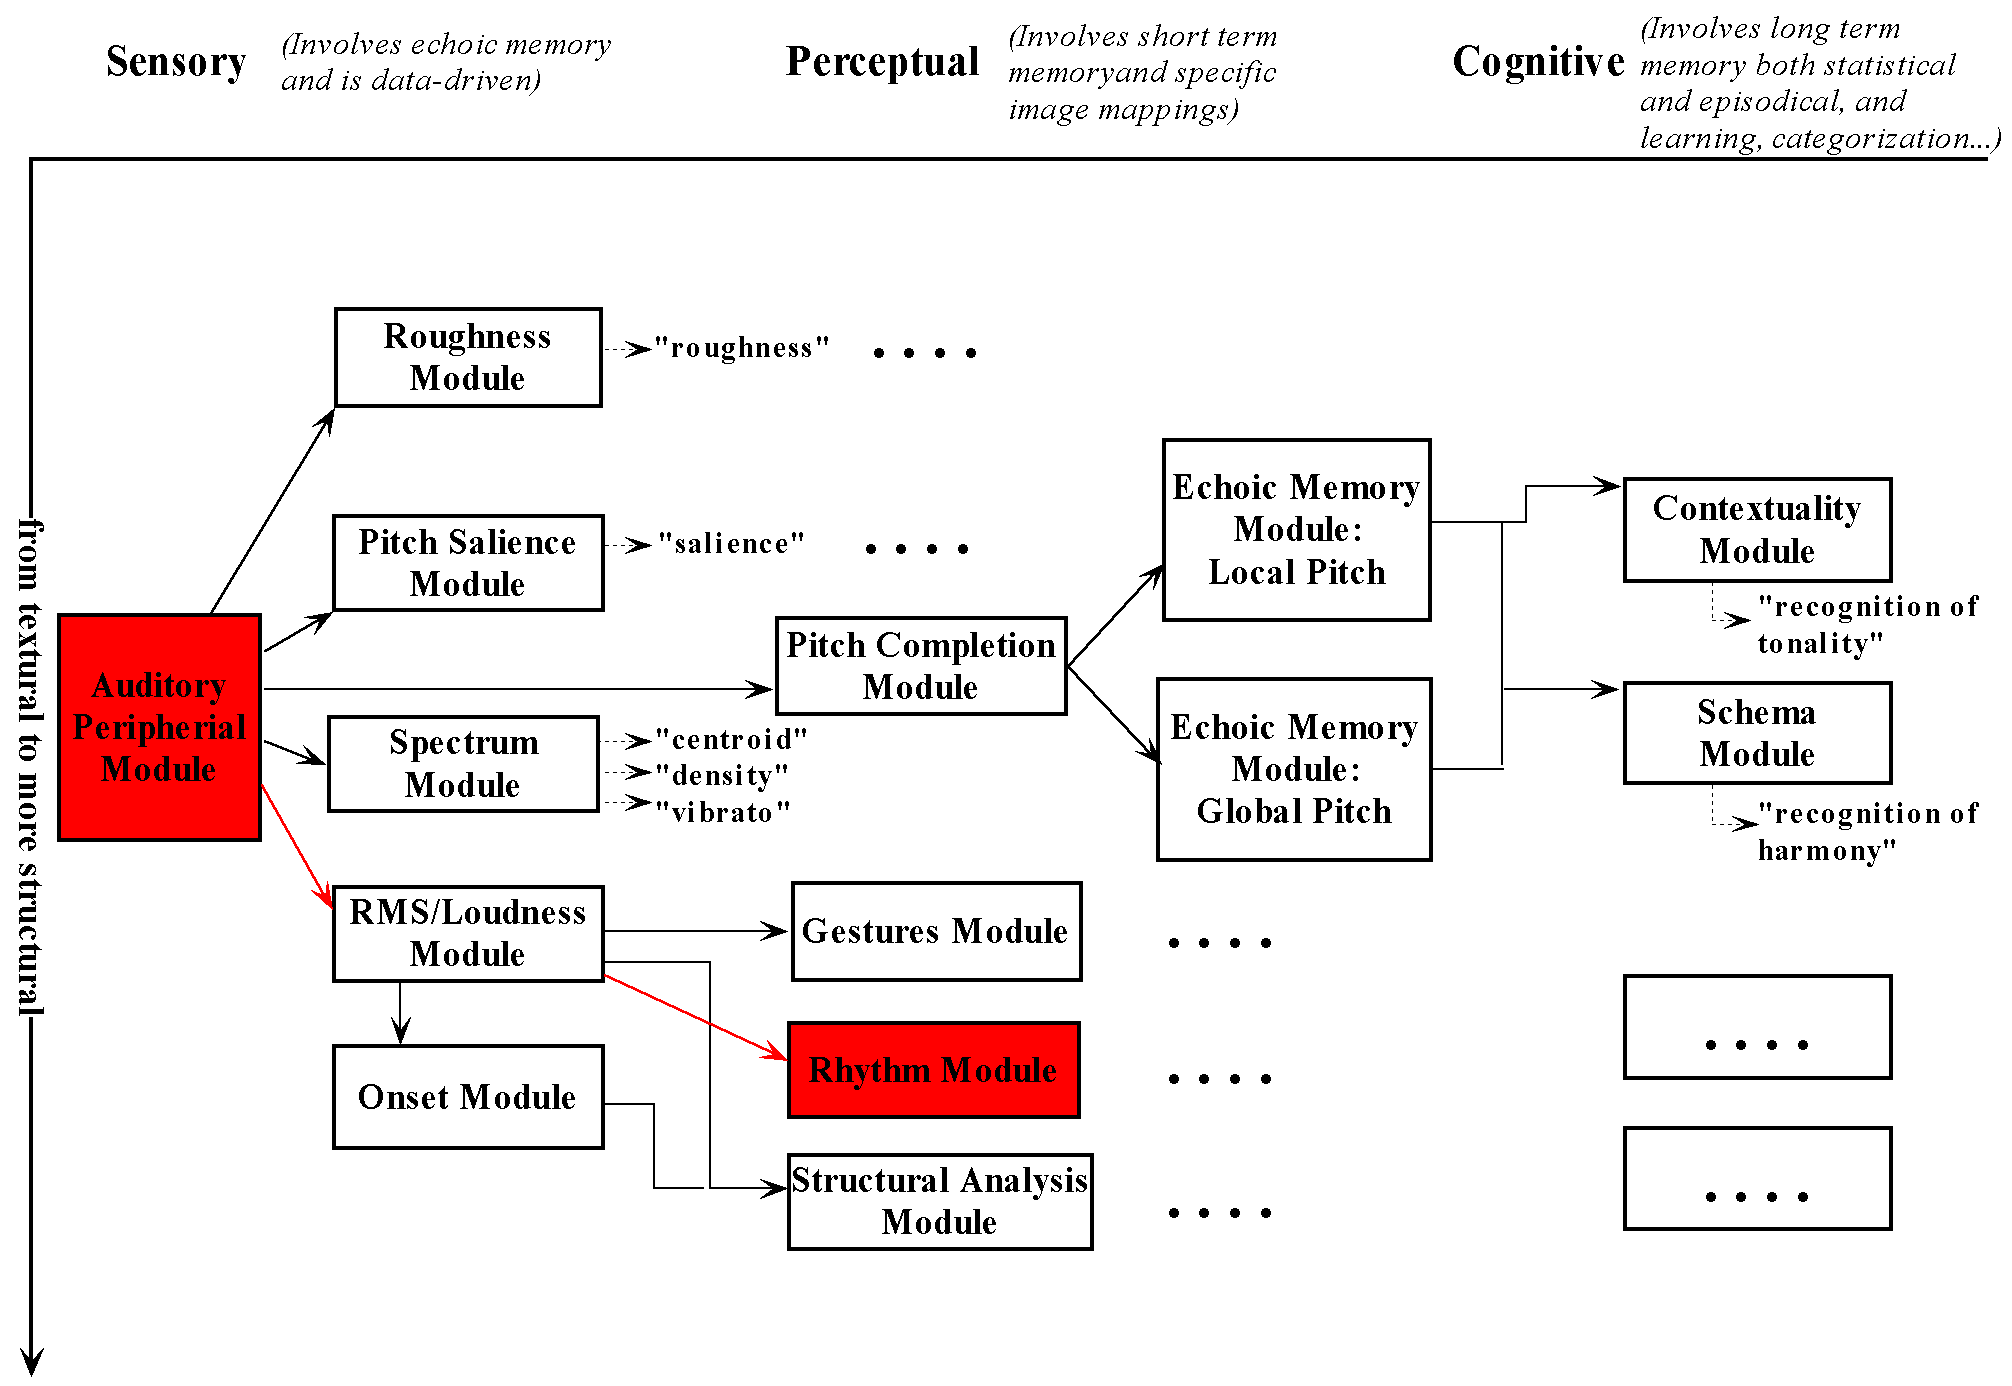
\includegraphics[width=\textwidth]{Graphics/ModulesRhM}
    \caption{Chart of image transformation modules, with RhM highlighted}
    \label{Fig:ModulesRhM}
\end{figure}


\subsection{Functional-logical description}
% --------------------------------------------------------------------------------

The Minimal Energy Change algorithm applied to the recognition of
repetition in rhythm involves:
\begin{eqnarray}
    APM: s(t) \rightarrow e(t,c)\\
    RMS: e(t,c) \rightarrow r(t,c)
\end{eqnarray}
where APM provides the auditory nerve images and where RMS
considers the energy in these images. The application of MEC
involves:
\begin{equation}
    MEC1:  r(t,c) \rightarrow m(\tau,t,c)
\end{equation}
where MEC1 performs a periodicity analysis of these energies and
outputs the estimated periodicity patterns $m(\tau,t,c)$, where
$t$ is time as usual, $\tau$ is the period, and $c$ is the
auditory channel. To obtain the summary MEC-analysis, one has to
sum over all auditory channels, which gives:
\begin{equation}
    MEC2: m(\tau,t) = \sum_{c=1}^{C} m(\tau,t,c)~=~\tilde{m}(t)
\end{equation}
Hence, the MEC-function can be summarized as:
\begin{equation}
    MEC:  \tilde{r}(t) \rightarrow \tilde{m}(t)
\end{equation}
In this notation, one should take into account that the tilde
character, indicating a vector representation, applies to
different dimensions. The components of $\tilde{r}(t)$ are the
channels, while the components of $\tilde{m}(t)$ are the different
periods considered in the analysis. A derived value is the
so-called "best period" $p(t)$, which we obtain by taking the
minimum in each $\tilde{m}(t)$ for fixed $t$, hence:
\begin{equation}
    MEC:  \tilde{r}(t) \rightarrow \tilde{m}(t) \rightarrow p(t)
\end{equation}


\subsection{Signal processing description}
% --------------------------------------------------------------------------------

The MEC-algorithm takes a signal $s(t)$ and its shifted version
$s(t-\tau)$. It then calculates the difference between both
signals, takes the absolute value, and integrates the result:
\begin{equation}\label{MECM1}
    a(\tau,t)~=~
    \int_{0}^{t}~\left|~
    s(t'-\tau)-s(t') ~\right|~
    ~dt'
\end{equation}
where $a(\tau,t)$ at fixed $t$ contains an analysis for all
$\tau$. $\tau$ is typically chosen in the region of interest. For
rhythm detection, this may be from 400 ms to 1 s. The obtained
analysis $a(\tau,t)$ at fixed $t$ is then searched for a minimum:
\begin{equation}\label{MECM2}
    p(t) = ~min_{\tau>0}~a(\tau,t)
\end{equation}
which gives a value $p$ for the best period at each time step $t$.

In practice, we can build in more stability by leaky-integrating
the $a(\tau,t)$ over $t$:
\begin{equation}\label{MECM1B}
    a(\tau,t)~=~
    \int_{0}^{t}~\left|~
    s(t'-\tau)-s(t') ~\right|~
    e^{\beta(t-t')}~dt'
\end{equation}
and apply Expression \ref{MECM2}.

When applied to the signal in different auditory channels, the
calculation will be applied to each channel, thus giving
$a(\tau,t,c)$. To get the best period, one may calculate $p(t)$
using $\sum_{c=1}^{C}a(\tau,t,c)$.


\subsection{Implementation}
% --------------------------------------------------------------------------------

\begin{tabularx}{\linewidth}{llX}
\hyperlink{FuncRef:IPEMMECAnalysis}{IPEMMECAnalysis} & - & Performs a periodicity analysis of a (multi-channel) signal using the MEC model\\
\hyperlink{FuncRef:IPEMMECExtractPatterns}{IPEMMECExtractPatterns} & - & Extracts the best pattern from the original signal using the results of an IPEMMECAnalysis run\\
\hyperlink{FuncRef:IPEMMECReSynthUI}{IPEMMECReSynthUI} & - & User interface callback function for interactively handling the resynthesis of MEC analysis results\\
\hyperlink{FuncRef:IPEMMECSaveResults}{IPEMMECSaveResults} & - & Utility function that saves the results of IPEMMECExtractPatterns, so that resynthesis can still be done at a later date, after reloading this data\\
\hyperlink{FuncRef:IPEMMECSynthesis}{IPEMMECSynthesis} & - & Generates an AM modulated noise signal constructed from a repetition of the pattern found at the specified time moment\\
\end{tabularx}


\subsection{Examples}
% --------------------------------------------------------------------------------

The first steps involve the preparation of the signal in which we
want to look for periodicity. This is done by:\\

\begin{IPEMCodeEnvironment}
[ANI,ANIFreq,ANIFilterFreqs] = IPEMCalcANIFromFile('SchumannKurioseGeschichte.wav');
\newline [RMS,RMSFreq] = IPEMCalcRMS(ANI,ANIFreq,0.050,0.020);
\newline [Periods,Best,AnalysisFreq,Values] = IPEMMECAnalysis(RMS,RMSFreq,0.5,3,[],1.5);
\end{IPEMCodeEnvironment}\\

The MEC algorithm has stored the periods that were analyzed in
\IPEMCodeExtract{Periods}, the indices (into
\IPEMCodeExtract{Periods}) for the best periods found in each
channel in \IPEMCodeExtract{Best}, and all values $m(\tau,t,c)$ in
\IPEMCodeExtract{Values}. The data format of
\IPEMCodeExtract{Values} is described in
\hyperlink{FuncRef:IPEMMECAnalysis}{IPEMMECAnalysis}. Just to give
you an example of how to work with MATLAB, we sum over all
channels $c$ in the following way:\\

\begin{IPEMCodeEnvironment}
SummaryPeriodicity = zeros(size(Values\{1\}));
\newline for channel = 1:40;
\newline SummaryPeriodicity = SummaryPeriodicity + Values\{channel\};
\newline end
\end{IPEMCodeEnvironment}\\

The values in \IPEMCodeExtract{SummaryPeriodicity} contain the
periodicity analysis over all channels which can be visualized
using the MATLAB code:\\

\begin{IPEMCodeEnvironment}
figure;
\newline imagesc((0:size(SummaryPeriodicity,2)-1)/AnalysisFreq,Periods,SummaryPeriodicity);
\newline xlabel('Time (in s)'); ylabel('Period (in s)');
\newline axis xy; colormap(1-gray);
\end{IPEMCodeEnvironment}\\

We plot the best periods of the summary periodicity on top of the
image.\\

\begin{IPEMCodeEnvironment}
[M,I]=min(SummaryPeriodicity); hold on;
\newline plot((0:length(I)-1)/AnalysisFreq,Periods(I));
\end{IPEMCodeEnvironment}\\

The resulting graph should be similar to the one in figure
\ref{Fig:RhMDifferenceValuesSchumannn}.

\begin{figure}[h]
    \centering
    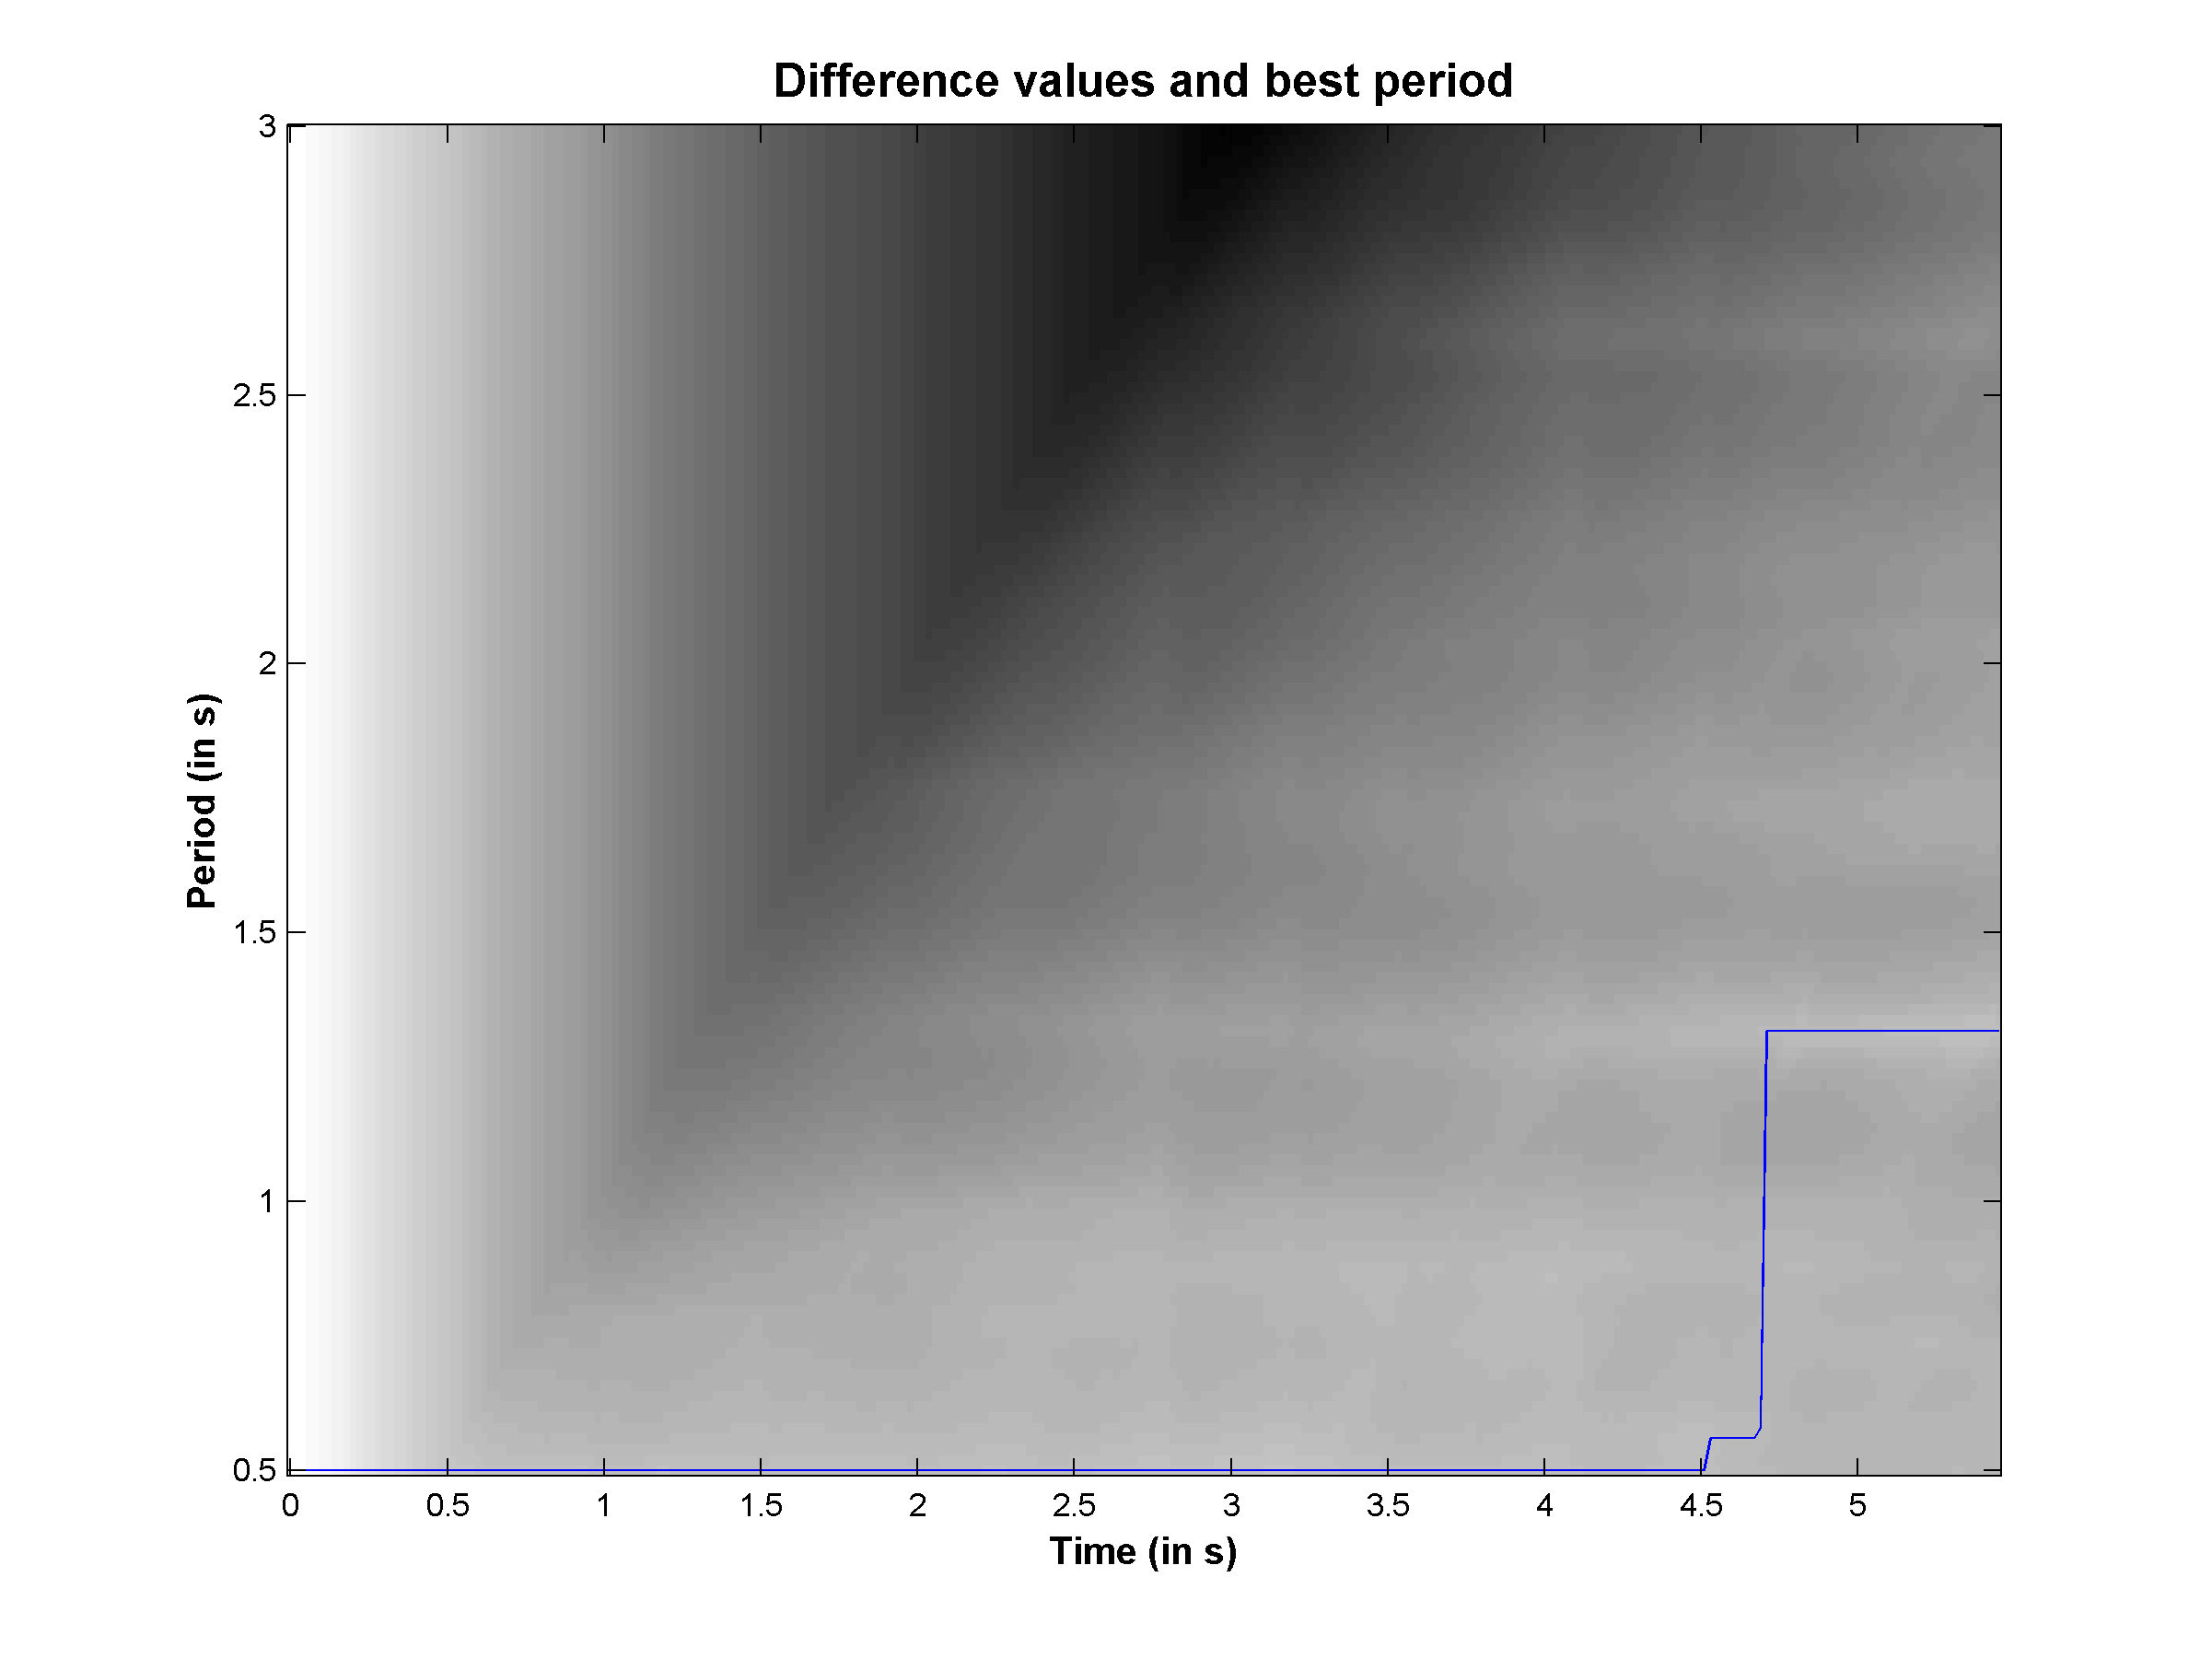
\includegraphics[width=\IPEMDefaultFigureWidth]{Graphics/RhMDifferenceValuesSchumannn}
    \caption{MEC analysis result of a short excerpt of Schumann's Kuriose Geschichte. Shown are the summed difference values (over all channels) and a plot of the best period on top of this.}
    \label{Fig:RhMDifferenceValuesSchumannn}
\end{figure}
